% Signed area under y=t on [0,1] is the triangle of area 1/2, beside four right rectangles.
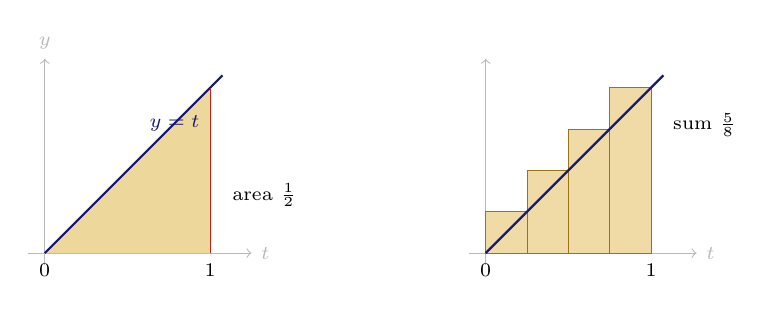
\begin{tikzpicture}[x=1.05cm,y=1.05cm]
  % left: triangle
  \begin{scope}
    \draw[gray!55,->] (-0.2,0) -- (2.5,0) node[right,font=\scriptsize] {$t$};
    \draw[gray!55,->] (0,-0.15) -- (0,2.35) node[above,font=\scriptsize] {$y$};
    \fill[Goldenrod!45] (0,0) -- (2,2) -- (2,0) -- cycle;
    \draw[MidnightBlue,thick] (0,0) -- (2.15,2.15);
    \draw[BrickRed,thin] (2,0) -- (2,2);
    \node[font=\scriptsize,anchor=north] at (0,-0.02) {$0$};
    \node[font=\scriptsize,anchor=north] at (2,-0.02) {$1$};
    \node[font=\scriptsize,MidnightBlue,anchor=south west] at (1.15,1.35) {$y=t$};
    \node[font=\scriptsize,anchor=west] at (2.15,0.7) {area $\frac12$};
  \end{scope}
  % right: four right-endpoint rectangles for y=t
  \begin{scope}[xshift=5.6cm]
    \draw[gray!55,->] (-0.2,0) -- (2.55,0) node[right,font=\scriptsize] {$t$};
    \draw[gray!55,->] (0,-0.15) -- (0,2.35);
    \foreach \k in {1,2,3,4} {
      \fill[Goldenrod!40] ({0.5*(\k-1)},0) rectangle ({0.5*\k},{0.5*\k});
      \draw[Goldenrod!70!black,thin] ({0.5*(\k-1)},0) rectangle ({0.5*\k},{0.5*\k});
    }
    \draw[MidnightBlue,thick] (0,0) -- (2.15,2.15);
    \node[font=\scriptsize,anchor=north] at (0,-0.02) {$0$};
    \node[font=\scriptsize,anchor=north] at (2,-0.02) {$1$};
    \node[font=\scriptsize,anchor=west] at (2.15,1.55) {sum $\frac58$};
  \end{scope}
\end{tikzpicture}
